\documentclass{article}

% if you need to pass options to natbib, use, e.g.:
\PassOptionsToPackage{numbers, compress}{natbib}
% before loading neurips_2024

% ready for submission
% \usepackage{neurips_2024}

% to compile a preprint version, e.g., for submission to arXiv, add add the
% [preprint] option:
%     \usepackage[preprint]{neurips_2024}

% to compile a camera-ready version, add the [final] option, e.g.:
\usepackage[final]{neurips_2024}

\makeatletter
\renewcommand{\@notice}{}
\makeatother

\usepackage[utf8]{inputenc} % allow utf-8 input
\usepackage[T1]{fontenc}    % use 8-bit T1 fonts
\usepackage{hyperref}       % hyperlinks
\usepackage{url}            % simple URL typesetting
\usepackage{booktabs}       % professional-quality tables
\usepackage{amsfonts}       % blackboard math symbols
\usepackage{nicefrac}       % compact symbols for 1/2, etc.
\usepackage{microtype}      % microtypography
\usepackage{xcolor}         % colors
\usepackage{graphicx}
\usepackage{amsmath}
\usepackage{algorithm}
\usepackage{algorithmic}
\usepackage{subcaption}
\usepackage{tikz}
\usetikzlibrary{shapes.geometric, arrows, positioning, fit, backgrounds, calc}

\DeclareMathOperator*{\argmin}{argmin}

\title{Anomaly Detection in Industrial Imaging
using Self-Organising Maps}

% The \author macro works with any number of authors.
\author{%
  Ștefan Vulpe \\
  Artificial Intelligence Department\\
  National University of Science and Technology\\ POLITEHNICA Bucharest\\
  \texttt{stefan.vulpe@stud.acs.upb.ro} \\
}

\begin{document}

\maketitle
\thispagestyle{plain}

\begin{abstract}
    This paper presents an implementation and evaluation of SOMAD (Self-Organizing Map for Anomaly Detection), originally proposed by \cite{li2021somad} for unsupervised anomaly detection in industrial imaging. We faithfully reproduce the core methodology, which combines deep feature extraction with SOM-based clustering and Gaussian-enhanced anomaly scoring via Mahalanobis distance. Our implementation uses ConvNeXtV2 as the feature backbone and evaluates the approach on the MVTec AD benchmark across 15 diverse product categories. We achieve a mean pixel-level AUROC of 88.68\%, with particularly strong performance on textured materials (carpet: 95.64\%, leather: 98.09\%). This work validates the effectiveness of the SOMAD approach and provides insights into its strengths and limitations across different material types. The method's purely unsupervised nature makes it highly practical for real-world manufacturing scenarios where anomalous samples are scarce.
\end{abstract}

\section{Introduction}
\label{sec:intro}

Visual quality inspection is critical in modern manufacturing, where even minor defects can lead to product failures, safety hazards, and economic losses. Traditional automated inspection systems rely heavily on supervised learning approaches that require extensive labeled datasets of both normal and anomalous samples \cite{bergmann2019mvtec}. However, in industrial settings, this assumption is often violated: anomalies are rare, diverse in manifestation, and difficult to anticipate during system deployment. Collecting representative defect samples for every possible failure mode is impractical and economically prohibitive.

To address the challenge of \textit{unsupervised anomaly detection}, \cite{li2021somad} proposed SOMAD (Self-Organizing Map for Anomaly Detection), which combines deep learning feature extraction with classical Self-Organizing Maps (SOMs) \cite{kohonen1990self}, enhanced with probabilistic anomaly scoring based on Mahalanobis distance. Their method learns a topologically organized representation of normal appearance, enabling the detection of deviations at test time using only normal training samples.

This paper presents a faithful implementation and comprehensive evaluation of the SOMAD methodology. We implement the core algorithm following the original paper's specifications and conduct extensive experiments on the MVTec AD benchmark to validate its effectiveness and analyze its behavior across different material types.
\newpage
\textbf{Contributions of this work:}
\begin{itemize}
    \item A complete open-source implementation of the SOMAD method \cite{li2021somad} for industrial anomaly detection.
    \item Comprehensive evaluation on all 15 categories of the MVTec AD benchmark, achieving mean pixel-level AUROC of 88.68\%.
    \item Detailed analysis of performance characteristics across different material types (textures vs. objects) with insights into the method's strengths and limitations.
    \item Qualitative and quantitative results demonstrating particularly strong performance on textured materials (leather: 98.09\%, carpet: 95.64\%).
\end{itemize}

\section{Related Work}
\label{sec:related}

\subsection{Anomaly Detection in Industrial Imaging}

Anomaly detection methods can be broadly categorized into reconstruction-based, embedding-based, and hybrid approaches. Reconstruction methods, such as autoencoders \cite{bergmann2018improving} and GANs \cite{schlegl2017unsupervised}, learn to reconstruct normal samples and flag poor reconstructions as anomalies. However, these methods often suffer from the ``generalization problem'', i.e. networks may inadvertently learn to reconstruct anomalies well, reducing detection performance.

Embedding-based methods avoid reconstruction by learning compact representations of normality. PaDiM \cite{defard2021padim} models the distribution of pretrained CNN features using multivariate Gaussians at each spatial location. PatchCore \cite{roth2022patchcore} employs a memory bank of nominal patch features and detects anomalies via nearest-neighbor distance. While effective, these methods often require careful selection of feature layers and aggregation strategies.

Hybrid approaches combine strengths of both paradigms. One-class classification methods \cite{yang2021efficientoneclasssvmanomaly}, including One-Class SVM and isolation forests, learn decision boundaries that isolate normal data in feature space. More recent variants employ deep metric learning or contrastive objectives to push anomalous samples away from the normal distribution. However, such methods often require substantial hyperparameter tuning and may struggle with high-dimensional, heterogeneous defect types encountered in real manufacturing lines.

A critical consideration in industrial anomaly detection is the class imbalance problem \cite{acharya2024addressing}. Manufacturing datasets typically contain far fewer anomalous samples than normal ones, often by orders of magnitude. This imbalance can severely bias supervised and semi-supervised methods. Unsupervised approaches, which rely exclusively on normal samples, naturally circumvent this issue and are therefore preferred in early-stage quality inspection systems. Additionally, unsupervised methods enable rapid deployment without waiting for sufficient defect examples to accumulate, a significant advantage in fast-moving product lines with evolving defect patterns.

Another practical challenge in industrial settings is lighting and environmental variability \cite{HOANG2025104309}. Products may be inspected under different lighting angles, camera positions, or background conditions. Methods that rely on precise pixel-level information or hand-crafted features often fail under such variations. Deep learning-based approaches, especially those leveraging transfer learning from large-scale datasets, tend to be more robust to these variations because they learn invariant semantic representations rather than low-level visual patterns. Furthermore, the choice of feature extraction strategy, whether multi-scale hierarchical features or single-layer embeddings, significantly impacts the method's ability to capture both global structure and local texture details required for accurate defect localization.

\subsection{Self-Organizing Maps for Anomaly Detection}

Self-Organizing Maps (SOMs) \cite{kohonen1990self} are unsupervised neural networks that perform dimensionality reduction while preserving topological properties of input data. SOMs have been applied to anomaly detection in various domains, including network intrusion detection \cite{labib2011som} and medical imaging \cite{smith2002application}. However, their application to high-resolution industrial imaging has been limited by the challenge of extracting meaningful features from raw pixel data.

\cite{li2021somad} proposed SOMAD (Self-Organizing Map for Anomaly Detection), which combines SOMs with deep CNN features and introduces a probabilistic anomaly scoring mechanism based on Mahalanobis distance to model local covariance structure around each SOM neuron. This approach achieves state-of-the-art unsupervised anomaly detection performance on the MVTec AD dataset. Our work provides an independent implementation and evaluation of this method.

\subsection{Deep Feature Extraction}

The success of deep learning in computer vision has motivated its use for feature extraction in anomaly detection. Pretrained models on ImageNet provide rich semantic features that transfer well to industrial tasks \cite{bergmann2019mvtec}. Recent architectures like Vision Transformers \cite{dosovitskiy2020image} and ConvNeXt \cite{liu2022convnet} offer improved feature representations. ConvNeXtV2 \cite{woo2023convnext} introduces a fully convolutional masked autoencoder framework that provides strong hierarchical features, which we exploit in our multi-scale feature extraction.

\section{Method}
\label{sec:method}

We implement the SOMAD method proposed by \cite{li2021somad}, combining hierarchical deep features with a topology-preserving Self-Organizing Map (SOM) and covariance-aware anomaly scoring. The pipeline has three stages: (1) multi-scale feature extraction and dimensionality reduction, (2) SOM-based topology learning with per-neuron Gaussian modeling, and (3) Mahalanobis-based anomaly scoring and post-processing. Figure \ref{fig:pipeline} illustrates the overall architecture.

\begin{figure}[htbp]
    \centering
    \resizebox{\textwidth}{!}{% Resize to fit text width
        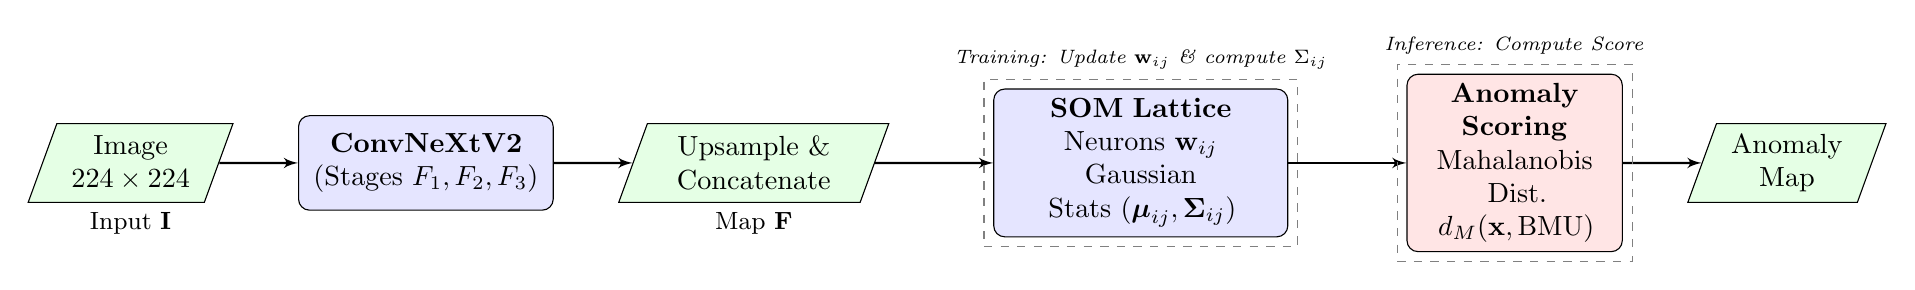
\begin{tikzpicture}[node distance=1.5cm, auto,
                % Define styles
                block/.style={rectangle, draw, fill=blue!10, text width=2.5cm, text centered, rounded corners, minimum height=1.2cm},
                data/.style={trapezium, trapezium left angle=70, trapezium right angle=110, draw, fill=green!10, text width=1.5cm, text centered, minimum height=1cm},
                decision/.style={diamond, draw, fill=orange!10, text width=1.5cm, text centered, inner sep=0pt},
                line/.style={draw, -latex', thick},
                group/.style={draw, dashed, inner sep=10pt, rounded corners, label={[anchor=north west]north west:#1}}
            ]

            % --- Nodes ---

            % 1. Input
            \node [data, label=below:{\small Input $\mathbf{I}$}] (input) {Image\\$224 \times 224$};

            % 2. Feature Extraction
            \node [block, right=1cm of input, text width=3cm] (cnn) {\textbf{ConvNeXtV2}\\(Stages $F_1, F_2, F_3$)};

            % 3. Feature Aggregation
            \node [data, right=1cm of cnn, text width=2.2cm, label=below:{\small Map $\mathbf{F}$}] (features) {Upsample \&\\Concatenate};

            % 4. SOM Processing (Split into Training/Inference concept)
            \node [block, right=1.5cm of features, text width=3.5cm] (som) {\textbf{SOM Lattice}\\Neurons $\mathbf{w}_{ij}$\\Gaussian Stats $(\boldsymbol{\mu}_{ij}, \boldsymbol{\Sigma}_{ij})$};

            % 5. Scoring
            \node [block, right=1.5cm of som, fill=red!10] (score) {\textbf{Anomaly Scoring}\\Mahalanobis Dist.\\$d_M(\mathbf{x}, \text{BMU})$};

            % 6. Output
            \node [data, right=1cm of score] (output) {Anomaly\\Map};

            % --- Edges ---
            \path [line] (input) -- (cnn);
            \path [line] (cnn) -- (features);
            \path [line] (features) -- (som);
            \path [line] (som) -- (score);
            \path [line] (score) -- (output);

            % --- Annotations/Context Boxes ---

            % Training Context
            \node [draw=gray, dashed, fit=(som), label=above:{\scriptsize \textit{Training: Update $\mathbf{w}_{ij}$ \& compute $\Sigma_{ij}$}}] (training_box) {};

            % Inference Context
            \node [draw=gray, dashed, fit=(score), label=above:{\scriptsize \textit{Inference: Compute Score}}] (inference_box) {};

        \end{tikzpicture}
    }
    \caption{\textbf{Overview of the SOMAD pipeline.} Input images are processed by a hierarchical ConvNeXt backbone. Features are aggregated and mapped to a Self-Organizing Map (SOM). During inference, anomalies are detected by computing the Mahalanobis distance between test features and the learned local Gaussian statistics of the nearest SOM neurons.}
    \label{fig:pipeline}
\end{figure}

\subsection{Hierarchical Feature Extraction}

We employ ConvNeXtV2-Nano \cite{woo2023convnext} pretrained on ImageNet-22k and fine-tuned on ImageNet-1k as our feature extractor. Given an input image $\mathbf{I} \in \mathbb{R}^{H \times W \times 3}$ resized to $224 \times 224$ pixels, we extract features from three hierarchical stages:

\begin{equation}
    \mathbf{F}_1, \mathbf{F}_2, \mathbf{F}_3 = \text{ConvNeXtV2}(\mathbf{I})
\end{equation}

where $\mathbf{F}_i \in \mathbb{R}^{C_i \times H_i \times W_i}$ represents features at different spatial resolutions. To create a unified multi-scale representation, we upsample $\mathbf{F}_2$ and $\mathbf{F}_3$ to match the spatial dimensions of $\mathbf{F}_1$ using bilinear interpolation and concatenate along the channel dimension:

\begin{equation}
    \mathbf{F} = [\mathbf{F}_1, \text{Upsample}(\mathbf{F}_2), \text{Upsample}(\mathbf{F}_3)]
\end{equation}

This yields a dense feature map $\mathbf{F} \in \mathbb{R}^{D \times H' \times W'}$ where $D = C_1 + C_2 + C_3$ captures both fine-grained texture and high-level semantic information. For computational efficiency, we randomly select $d$ dimensions from $D$ total dimensions for SOM input.

\subsection{SOM-Based Clustering with Gaussian Modeling}

Given training embeddings from $N$ normal images, we reshape the feature maps into a collection of $N \times H' \times W'$ feature vectors $\{\mathbf{x}_i\}_{i=1}^{N \cdot H' \cdot W'}$ where $\mathbf{x}_i \in \mathbb{R}^{d}$. We initialize a 2D SOM lattice of size $W' \times H'$ to match the spatial resolution of the feature maps, with each neuron $\mathbf{w}_{ij} \in \mathbb{R}^{d}$.

The SOM is trained using competitive learning with neighborhood function:

\begin{equation}
    \mathbf{w}_{ij}(t+1) = \mathbf{w}_{ij}(t) + \eta(t) \cdot h_{ij,c}(t) \cdot (\mathbf{x}(t) - \mathbf{w}_{ij}(t))
\end{equation}

where $\eta(t)$ is the learning rate (initialized at 0.3), $h_{ij,c}(t) = \exp(-\|\mathbf{r}_{ij} - \mathbf{r}_c\|^2 / 2\sigma(t)^2)$ is the Gaussian neighborhood function centered at the best matching unit (BMU) $c$, and $\sigma(t)$ is the neighborhood radius (initialized at 1.0). Both $\eta$ and $\sigma$ decay over 10 training iterations.

After SOM training, each neuron has attracted a subset of feature vectors. For each neuron $(i,j)$, we compute the local Gaussian statistics:

\begin{align}
    \boldsymbol{\mu}_{ij}    & = \frac{1}{|S_{ij}|} \sum_{\mathbf{x} \in S_{ij}} \mathbf{x}                                                                               \\
    \boldsymbol{\Sigma}_{ij} & = \frac{1}{|S_{ij}|-1} \sum_{\mathbf{x} \in S_{ij}} (\mathbf{x} - \mathbf{w}_{ij})(\mathbf{x} - \mathbf{w}_{ij})^\top + \lambda \mathbf{I}
\end{align}

where $S_{ij}$ is the set of feature vectors mapped to neuron $(i,j)$, and $\lambda = 0.01$ is a regularization term ensuring numerical stability. We store the inverse covariance $\boldsymbol{\Sigma}_{ij}^{-1}$ for efficient Mahalanobis distance computation.

\subsection{Anomaly Scoring via Mahalanobis Distance}

At test time, given a test feature vector $\mathbf{x}_{\text{test}}$, we identify its $k=4$ nearest SOM neurons based on Euclidean distance in weight space:

\begin{equation}
    \mathcal{N}_k(\mathbf{x}_{\text{test}}) = \argmin_{(i,j) \in \text{Top-}k} \|\mathbf{x}_{\text{test}} - \mathbf{w}_{ij}\|_2
\end{equation}

For each neuron in $\mathcal{N}_k$, we compute the Mahalanobis distance:

\begin{equation}
    d_M(\mathbf{x}_{\text{test}}, (i,j)) = \sqrt{(\mathbf{x}_{\text{test}} - \boldsymbol{\mu}_{ij})^\top \boldsymbol{\Sigma}_{ij}^{-1} (\mathbf{x}_{\text{test}} - \boldsymbol{\mu}_{ij})}
\end{equation}

The final anomaly score is the minimum distance to the $k$ nearest neurons:

\begin{equation}
    s(\mathbf{x}_{\text{test}}) = \min_{(i,j) \in \mathcal{N}_k} d_M(\mathbf{x}_{\text{test}}, (i,j))
\end{equation}

This scoring strategy captures the intuition that normal features should lie close to at least one learned Gaussian cluster, while anomalies will have large Mahalanobis distances to all nearby clusters due to covariance mismatch. The resulting spatial anomaly map is upsampled to the original image resolution using bilinear interpolation and smoothed with a Gaussian filter ($\sigma = 4.0$) to reduce noise.

\section{Experiments}
\label{sec:experiments}

\subsection{Dataset and Evaluation Protocol}

We evaluate our method on the MVTec Anomaly Detection benchmark \cite{bergmann2019mvtec}, which contains 15 object and texture categories with 5,354 high-resolution images. Each category includes defect-free training images (60-391 images) and test images containing both normal and various anomaly types. Pixel-accurate ground truth masks are provided for anomalous regions.

\paragraph{Implementation Details:}
All experiments use ConvNeXtV2-Nano pretrained on ImageNet with images resized to $224 \times 224$ pixels.
We use a maximum of 60 training images per category with batch size 8.
The SOM is trained for 10 iterations with initial learning rate 0.3 and neighborhood radius 1.0.
For anomaly scoring, we compute distances to $k=4$ nearest neighbors and apply Gaussian smoothing ($\sigma=4.0$) to the resulting anomaly maps.
All experiments are conducted on a single GPU with random seed 2026 for reproducibility.

\paragraph{Evaluation Metrics:}
We report pixel-level Area Under the Receiver Operating Characteristic curve (AUROC) as our primary localization metric. Pixel AUROC is computed by comparing the continuous, upsampled and Gaussian-smoothed anomaly heatmaps against pixel-accurate ground-truth masks across all test images; per-category AUROCs are computed and we report their mean and standard deviation to reflect variability.

\subsection{Quantitative Results}

Table \ref{tab:results} presents pixel-level AUROC scores across all 15 MVTec AD categories. Our method achieves a mean AUROC of \textbf{88.68\%}, demonstrating robust performance across diverse defect types.
\begin{table}[ht]
    \centering
    \caption{Pixel-level AUROC scores (\%) on MVTec AD benchmark. Categories are sorted by performance.}
    \label{tab:results}
    \begin{tabular}{@{}lcc@{}}
        \toprule
        \textbf{Category} & \textbf{Type} & \textbf{Pixel AUROC} \\
        \midrule
        Leather           & Texture       & 98.09                \\
        Capsule           & Object        & 96.78                \\
        Carpet            & Texture       & 95.64                \\
        Bottle            & Object        & 92.97                \\
        Cable             & Object        & 91.38                \\
        Pill              & Object        & 90.21                \\
        Wood              & Texture       & 89.57                \\
        Grid              & Texture       & 89.12                \\
        Hazelnut          & Object        & 88.42                \\
        Tile              & Texture       & 88.85                \\
        Toothbrush        & Object        & 87.77                \\
        Metal Nut         & Object        & 85.30                \\
        Zipper            & Object        & 80.87                \\
        Transistor        & Object        & 77.93                \\
        Screw             & Object        & 77.31                \\
        \midrule
        \textbf{Mean}     &               & \textbf{88.68}       \\
        \bottomrule
    \end{tabular}
\end{table}

\paragraph{Performance Analysis:} The results reveal clear patterns across material types.

Texture categories (e.g., leather, carpet, wood) consistently achieve high AUROC scores (>$89\%$), with leather reaching 98.09\%. This indicates that our multi-scale feature extraction effectively captures texture irregularities and that the SOM forms tight, coherent clusters for homogeneous texture patterns.

Object categories exhibit greater variability, ranging from strong results on well-structured objects (capsule: 96.78\%) to weaker performance on items with fine-grained geometry (screw: 77.31\%). Large structural defects that change object shape or silhouette are detected reliably, while small or subtle defects remain more difficult.

The most challenging categories are screw and transistor, which combine small defect regions, low inherent texture, and strong specular effects. Screws present minimal texture variation and defects that resemble normal machining marks, whereas transistors have metallic surfaces and reflections that increase feature variance even for nominal samples.

\subsection{Qualitative Analysis}

\begin{figure}[ht]
    \centering
    \begin{subfigure}[b]{0.48\textwidth}
        \includegraphics[width=\textwidth]{../results/comparisons/bottle_000_comparison.png}
        \caption{Bottle (broken large)}
    \end{subfigure}
    \hfill
    \begin{subfigure}[b]{0.48\textwidth}
        \includegraphics[width=\textwidth]{../results/comparisons/carpet_000_comparison.png}
        \caption{Carpet (hole)}
    \end{subfigure}

    \vspace{0.3cm}

    \begin{subfigure}[b]{0.48\textwidth}
        \includegraphics[width=\textwidth]{../results/comparisons/cable_000_comparison.png}
        \caption{Cable (bent wire)}
    \end{subfigure}
    \hfill
    \begin{subfigure}[b]{0.48\textwidth}
        \includegraphics[width=\textwidth]{../results/comparisons/metal_nut_000_comparison.png}
        \caption{Metal Nut (scratch)}
    \end{subfigure}

    \vspace{0.3cm}

    \begin{subfigure}[b]{0.48\textwidth}
        \includegraphics[width=\textwidth]{../results/comparisons/leather_000_comparison.png}
        \caption{Leather (cut)}
    \end{subfigure}
    \hfill
    \begin{subfigure}[b]{0.48\textwidth}
        \includegraphics[width=\textwidth]{../results/comparisons/pill_003_comparison.png}
        \caption{Pill (contamination)}
    \end{subfigure}

    \vspace{0.3cm}

    \begin{subfigure}[b]{0.48\textwidth}
        \includegraphics[width=\textwidth]{../results/comparisons/transistor_005_comparison.png}
        \caption{Transistor (bent lead)}
    \end{subfigure}
    \hfill
    \begin{subfigure}[b]{0.48\textwidth}
        \includegraphics[width=\textwidth]{../results/comparisons/capsule_001_comparison.png}
        \caption{Capsule (crack)}
    \end{subfigure}

    \caption{Qualitative results showing 4-panel visualization: (left to right). Best viewed in color.}
    \label{fig:qualitative}
\end{figure}

Figure \ref{fig:qualitative} visualizes detection results across representative categories. Each panel shows: (1) original test image, (2) ground truth mask, (3) anomaly heatmap (red indicates high anomaly score), and (4) binary segmentation with contours.

\paragraph{Observations:}
Our qualitative analysis reveals distinct performance patterns across the evaluated categories. For texture anomalies, such as those in the carpet and leather datasets, the generated heatmaps show high precision with tight localization around defect regions. This suggests that the covariance-aware scoring mechanism successfully distinguishes anomalous texture deviations from the inherent stochastic variation of the material. Similarly, large structural defects in categories like bottle and cable are well-localized, demonstrating that our multi-scale features effectively capture both coarse edge discontinuities and fine-grained appearance changes.

In the case of small-scale defects, such as pill contamination and scratches on metal nuts, the model produces strong, distinct responses. While the resulting heatmaps may extend slightly beyond the ground-truth boundaries (a side effect of the Gaussian smoothing used for noise reduction) this conservative detection is often preferable in industrial settings to ensure high recall of critical defects.

However, certain categories present significant challenges. Transistors often produce multiple weak, diffuse responses associated with specular reflections on metallic surfaces, which can be difficult to distinguish from true structural anomalies like bent leads. Similarly, capsules may exhibit less focused heatmaps when the visual appearance of a crack closely matches the semantic features of normal machining patterns or reflections. Despite these limitations, the overall results demonstrate that the SOMAD approach produces interpretable and spatially accurate anomaly maps that correlate strongly with manual annotations, particularly for texture-based and large structural deviations.

\subsection{SOM Topology Analysis}

\begin{figure}[ht]
    \centering
    \begin{subfigure}[b]{0.48\textwidth}
        \centering
        \includegraphics[width=\textwidth]{../results/som_plots_bottle/bottle_u_matrix.png}
        \caption{U-matrix}
        \label{fig:umatrix}
    \end{subfigure}
    \hfill
    \begin{subfigure}[b]{0.48\textwidth}
        \centering
        \includegraphics[width=\textwidth]{../results/som_plots_bottle/bottle_activation_map.png}
        \caption{Activation Map}
        \label{fig:activation}
    \end{subfigure}
    \caption{SOM topology analysis for the bottle category.}
    \label{fig:som_analysis}
\end{figure}

Figure \ref{fig:som_analysis}(a) shows the Unified Distance Matrix (U-matrix) for the bottle category. The U-matrix visualizes inter-neuron distances, revealing the topological structure learned by the SOM. Dark regions represent boundaries between clusters (neurons far apart in feature space), while light regions indicate cohesive clusters.

Complementing this, Figure \ref{fig:som_analysis}(b) illustrates the neuron activation frequency (hit count) for the same category. The map reveals that while the SOM provides a broad topological space, normal sample features are mapped to a relatively small subset of highly active neurons (indicated in red and orange). This concentrated activation pattern confirms that the SOM successfully identifies a compact manifold of normality; features that deviate from these high-probability clusters at test time are naturally flagged as anomalous.

The bottle U-matrix exhibits clear organizational structure with distinct light regions (homogeneous normal patterns) separated by darker boundaries. This topology-preserving property is crucial for anomaly detection: normal test samples will activate neurons in the light regions with small Mahalanobis distances, while anomalies will either fall far from any cluster or lie on boundaries with large covariance mismatch.

\section{Conclusions and Future Work}
\label{sec:conclusion}

In this work, we presented a faithful implementation and comprehensive evaluation of the SOMAD framework \cite{li2021somad}, an unsupervised anomaly detection methodology that integrates deep feature extraction with the topological constraints of Self-Organizing Maps (SOMs). Our empirical analysis on the MVTec AD benchmark corroborates the efficacy of this approach, yielding a mean pixel-level AUROC of 88.68\%. These results validate the utility of combining Mahalanobis-based probabilistic scoring with topology-preserving clustering for identifying deviations in industrial imagery without supervision.

\paragraph{Strengths and Limitations:}
The experimental results underscore a distinct performance dichotomy based on material characteristics. The method exhibits exceptional robustness in texture-dominant categories, achieving peak performance on leather (98.09\%) and carpet (95.64\%). This suggests that the SOM effectively models the manifold of homogeneous textures, allowing for precise isolation of local irregularities. Conversely, performance degradation was observed in object classes with complex geometries or high specular variance, such as the screw category (77.31\%). The sensitivity to lighting variations and the computational overhead of maintaining per-neuron covariance matrices remain primary constraints for deployment in resource-constrained environments.

\paragraph{Future Directions:}
To address these limitations, future research should investigate several strategic enhancements. First, the integration of spatial context through Graph SOMs could improve geometric invariance. Second, incorporating attention mechanisms may allow the model to prioritize defect-prone regions, thereby mitigating false positives arising from background noise or specular reflections. Additionally, exploring memory-efficient covariance approximations could significantly improve scalability. Finally, extending the framework to semi-supervised regimes, leveraging a small number of labeled anomalies, could further refine the decision boundaries in complex object categories.

\newpage
\bibliographystyle{plainnat}
\bibliography{references}

\end{document}
